
In this section we summarise the results obtained using the shape analysis based on the 
matrix element output. 
Tables~\ref{tab:yield_me_shapebased} shows the signal and 
equivalent data yields and background expectations in ee and $\mu\mu$ final states respectively. 
Figure~\ref{fig:histo_me_250_5fb}-\ref{fig:histo_me_600_5fb} show the matrix element output distribution 
after the higgs mass dependent selections, for the mass hypothesis between 250 and 600 $\GeV$, 
corresponding to \intlumi. In these figures the background normalizations are scaled by 
each individual data-to-mc scale factors to account for the data and MC difference in 
background estimation described in section~\ref{sec:backgrounds}, 
lepton efficiency and the pileup reweighting. 


The expected cross section ratio limits as a function of the Higgs mass, together with the 1/2-$\sigma$ uncertainty 
bands are shown in Table~\ref{tab:limits_meshape_5fb} and Figure~\ref{fig:limits_meshape_5fb}. 
The observed exclusion region for the Standard Model Higgs is [300,500]~\GeV{} at 95\%C.L., 
compared to the expected exclusion region as [280,480]~\GeV{} at 95\%C.L.
Compared to the cut-based analysis, performing shape analysis based on the matrix element output 
improves the search sensitivity by upto $20\%$. 

%Performing shape analysis based on the matrix element output variable 
%improves the search sensitivity by about $10-15\%$, ignoring the systematics due to the 
%uncertainties of shape variations. Including the uncertainties due to the shape variations 
%degrades the performance degrade by up to 6\%. 

%%%%%%%%%%%%%%%%%%%%%%%%%
\begin{table}[!ht]
{\scriptsize
 \begin{center}
 \begin{tabular}{l | c c | c c c c c c | c}
 \hline\hline
 $mH$ & qqH & ggH & ZZ & ggZZ & WZ & WW/Top & Zjets & $\sum$Bkg & Data \\
 \hline
\multicolumn{10}{c} {ee} \\ 
\hline
250 & $1.1\pm0.1$ & $8.9\pm1.3$ & $27.4\pm2.9$ & $2.4\pm0.5$ & $18.7\pm2.3$ & $54.7\pm4.9$ & $18.9\pm18.9$ & $122.7\pm19.9$ & 115 \\
300 & $1.2\pm0.1$ & $10.3\pm1.6$ & $22.4\pm2.4$ & $2.0\pm0.4$ & $14.3\pm1.8$ & $38.9\pm4.2$ & $11.5\pm11.5$ & $89.6\pm12.6$ & 84 \\
350 & $1.0\pm0.1$ & $10.8\pm1.7$ & $18.2\pm1.9$ & $1.6\pm0.4$ & $10.6\pm1.3$ & $22.6\pm3.2$ & $8.1\pm8.1$ & $61.7\pm9.0$ & 58 \\
400 & $0.7\pm0.1$ & $9.3\pm1.6$ & $18.2\pm1.9$ & $1.6\pm0.4$ & $10.6\pm1.3$ & $22.6\pm3.2$ & $8.1\pm8.1$ & $61.7\pm9.0$ & 58 \\
500 & $0.4\pm0.1$ & $4.2\pm1.0$ & $14.8\pm1.6$ & $1.3\pm0.3$ & $8.0\pm1.0$ & $14.3\pm2.5$ & $5.9\pm5.9$ & $44.8\pm6.7$ & 47 \\
600 & $0.2\pm0.1$ & $1.6\pm0.6$ & $9.9\pm1.1$ & $0.8\pm0.2$ & $4.6\pm0.6$ & $3.6\pm1.3$ & $3.4\pm3.4$ & $22.4\pm3.9$ & 26 \\
\hline
\multicolumn{10}{c} {$\mu\mu$} \\ 
\hline
250 & $1.5\pm0.1$ & $12.8\pm1.8$ & $40.3\pm3.9$ & $3.6\pm0.8$ & $27.6\pm3.2$ & $68.1\pm6.1$ & $27.9\pm27.9$ & $167.9\pm29.1$ & 173 \\
300 & $1.7\pm0.1$ & $14.8\pm2.2$ & $33.2\pm3.2$ & $2.9\pm0.6$ & $20.8\pm2.5$ & $48.1\pm5.2$ & $17.1\pm17.1$ & $122.6\pm18.3$ & 125 \\
350 & $1.4\pm0.1$ & $15.3\pm2.4$ & $26.8\pm2.6$ & $2.3\pm0.5$ & $15.6\pm1.8$ & $28.2\pm3.9$ & $12.0\pm12.0$ & $85.4\pm13.1$ & 89 \\
400 & $1.0\pm0.1$ & $13.3\pm2.3$ & $26.8\pm2.6$ & $2.3\pm0.5$ & $15.6\pm1.8$ & $28.2\pm3.9$ & $12.0\pm12.0$ & $85.4\pm13.1$ & 89 \\
500 & $0.6\pm0.1$ & $5.6\pm1.3$ & $21.6\pm2.1$ & $1.8\pm0.4$ & $11.8\pm1.4$ & $17.8\pm3.2$ & $8.8\pm8.8$ & $62.2\pm9.7$ & 63 \\
600 & $0.3\pm0.1$ & $2.3\pm0.8$ & $14.2\pm1.4$ & $1.2\pm0.3$ & $6.7\pm0.8$ & $4.5\pm1.6$ & $5.0\pm5.0$ & $31.7\pm5.5$ & 34 \\
\hline\hline
\end{tabular}
\end{center}
}
\caption{Expected number of signal and background events for an integrated luminosity of \intlumi after applying the higgs selections in the 
shape-based analysis based on matrix element output. Both statistical and systematic uncertainties are included. }
\label{tab:yield_me_shapebased}
\end{table}
%%%%%%%%%%%%%%%%%%%%%%%


%%%%%%%%%%%%%%%%%%%%%%%%%%%%%%%
\begin{table}[!ht]
\begin{center}
\begin{tabular}{ccccc}
\hline\hline
Mass & Observed & Median Expected & [-$\sigma$, +$\sigma$] & [-2$\sigma$, +2$\sigma$]\\\hline
250 & 1.21 & 1.31 & [0.95, 1.82] & [0.71, 2.42] \\
300 & 0.99 & 0.87 & [0.63, 1.21] & [0.47, 1.61] \\
350 & 0.63 & 0.64 & [0.46, 0.88] & [0.35, 1.17] \\
400 & 0.56 & 0.64 & [0.46, 0.89] & [0.35, 1.19] \\
500 & 1.00 & 1.13 & [0.81, 1.57] & [0.61, 2.08] \\
600 & 1.96 & 2.43 & [1.75, 3.37] & [1.32, 4.48] \\
\hline\hline
\end{tabular}
\end{center}
\caption{The observed and expected cross section ratio limits as a function 
of the Higgs mass, together with the 1/2-$\sigma$ uncertainty bands obtained in the cut-and-count analysis, corresponding to 
an integrated luminosity of \intlumi}
\label{tab:limits_meshape_5fb}
\end{table}
%%%%%%%%%%%%%%%%%%%%%%%


%%%%%%%%%%%%%%%%%%%%%%%
\begin{table}
\begin{center}
{\normalsize
\begin{tabular}{|l|c|c|c|c|c|c|}
\hline
      &  \multicolumn{3}{c|}{ without shape uncertainty} &\multicolumn{3}{c|}{ with shape uncertainty} \\
\hline
Mass  &  Median      &     68\% C.L. band &  95\% C.L. band &  Median	   &	 68\% C.L. band &  95\% C.L. band\\
      &  Expected    &                    &                 &  Expected    &			&		 \\
\hline
250 & 1.32 & [0.96, 1.84] & [0.72, 2.44] & 1.31 & [0.95, 1.82] & [0.71, 2.42] \\
300 & 0.85 & [0.61, 1.18] & [0.46, 1.57] & 0.87 & [0.63, 1.21] & [0.47, 1.61] \\
350 & 0.64 & [0.46, 0.88] & [0.35, 1.18] & 0.64 & [0.46, 0.88] & [0.35, 1.17] \\
400 & 0.64 & [0.46, 0.89] & [0.35, 1.18] & 0.64 & [0.46, 0.89] & [0.35, 1.19] \\
500 & 1.13 & [0.82, 1.57] & [0.61, 2.09] & 1.13 & [0.82, 1.57] & [0.61, 2.09] \\
600 & 2.71 & [1.95, 3.76] & [1.47, 5.00] & 2.39 & [1.72, 3.32] & [1.30, 4.41] \\
\hline
\end{tabular}
}
\end{center}
\caption{The median expected cross section ratio limits as a function 
of the Higgs mass, together with the 1/2-$\sigma$ uncertainty bands obtained in the shape analysis based on matrix element output, 
corresponding to an integrated luminosity of \intlumi}
\label{tab:limits_meshape_uncert_5fb}
\end{table}
%%%%%%%%%%%%%%%%%%%%%%%


%%%%%%%%%%%%%%%%%%%%%%
\begin{figure}[!ht]
\begin{center}
   \subfigure[]{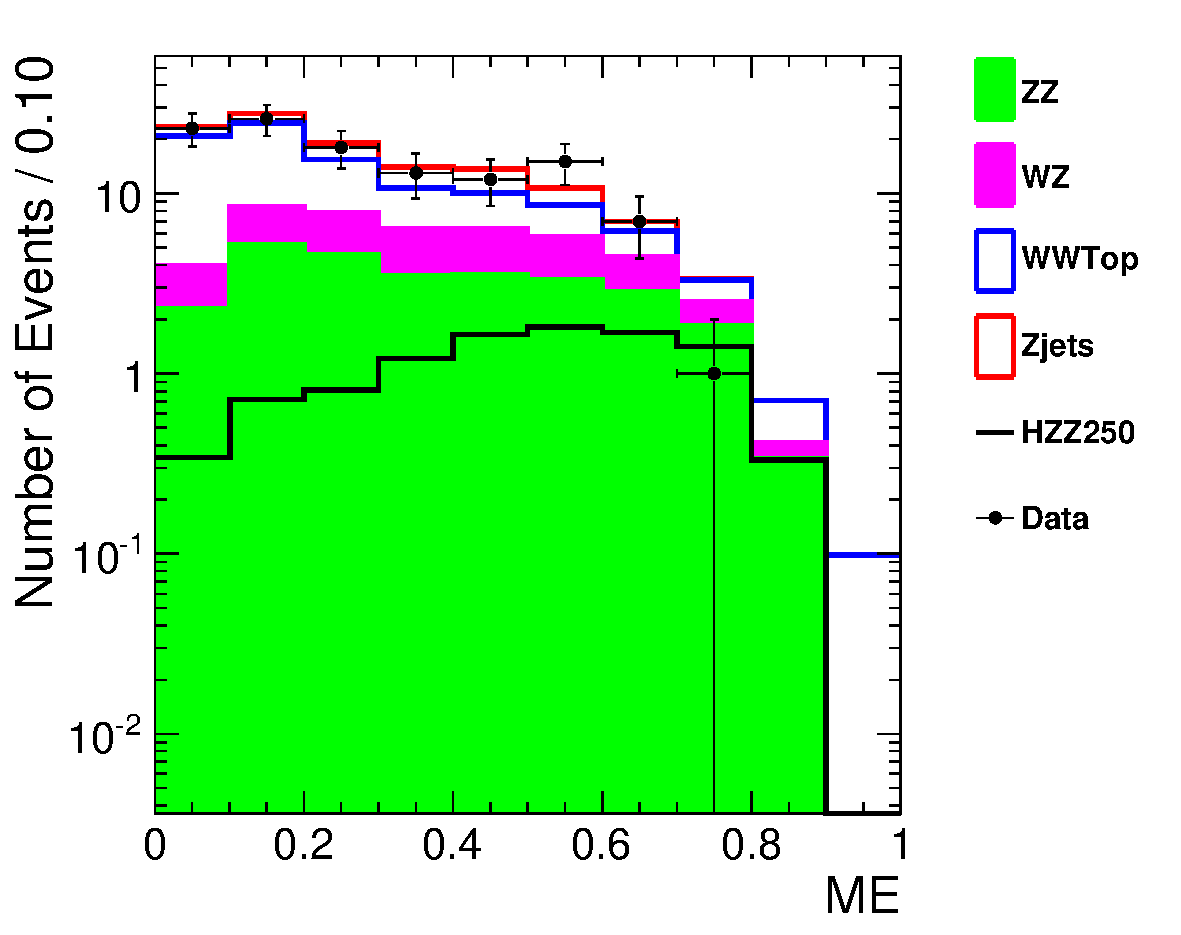
\includegraphics[width=0.4\textwidth,angle=0]{figures/ME_mH250_ee_stack_log.pdf}} 
   \subfigure[]{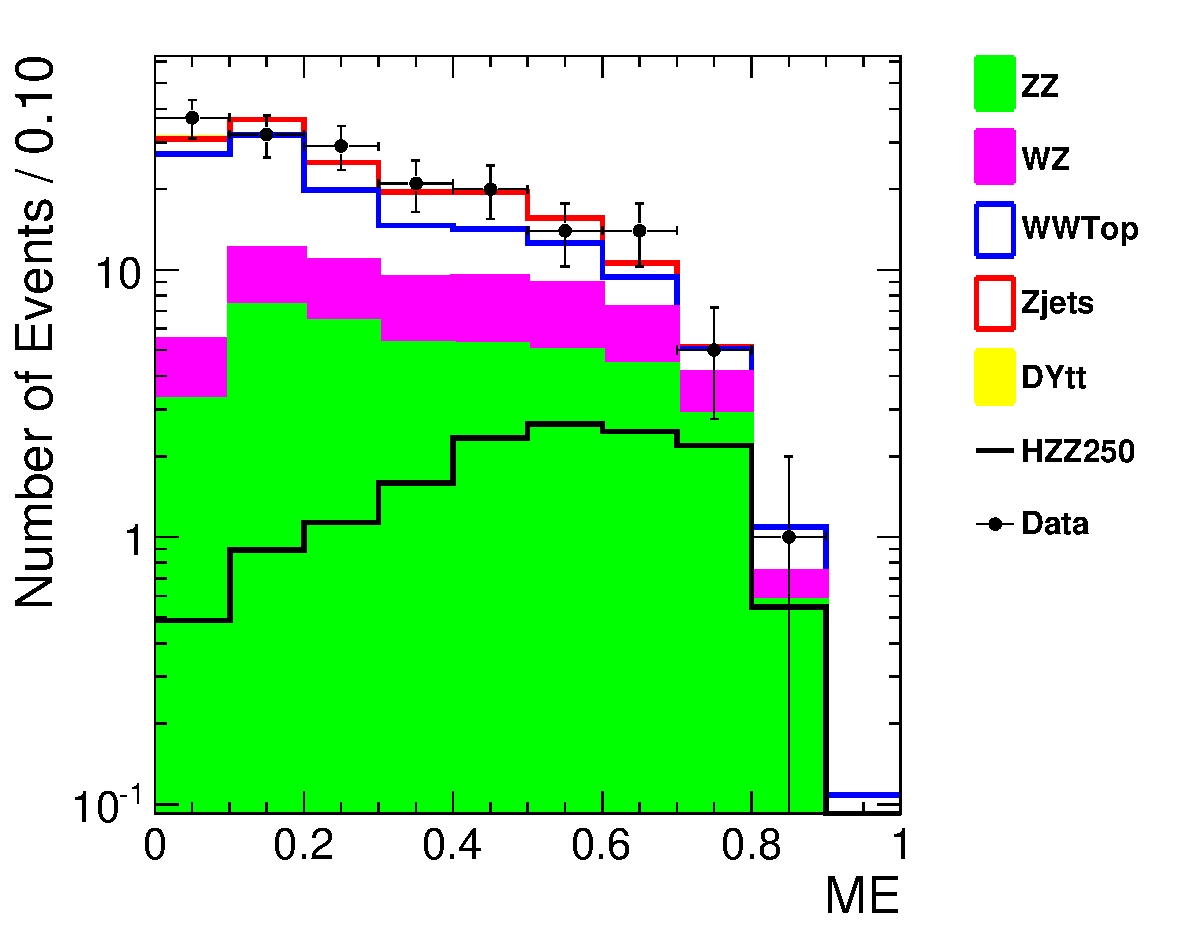
\includegraphics[width=0.4\textwidth,angle=0]{figures/ME_mH250_mm_stack_log.pdf}} \\ 
   \caption{The matrix element output distribution for Higgs signal and background events 
for \mHi=250 $\GeVcc$ in ee (a) and $\mu\mu$ final state (b) after the higgs dependent selections. 
The distributions are normalized to \intlumi with the background scaled by the data-to-mc ratios derived from data.}
   \label{fig:histo_me_250_5fb}
\end{center}
%\end{figure}

%\begin{figure}[!ht]
\begin{center}
   \subfigure[]{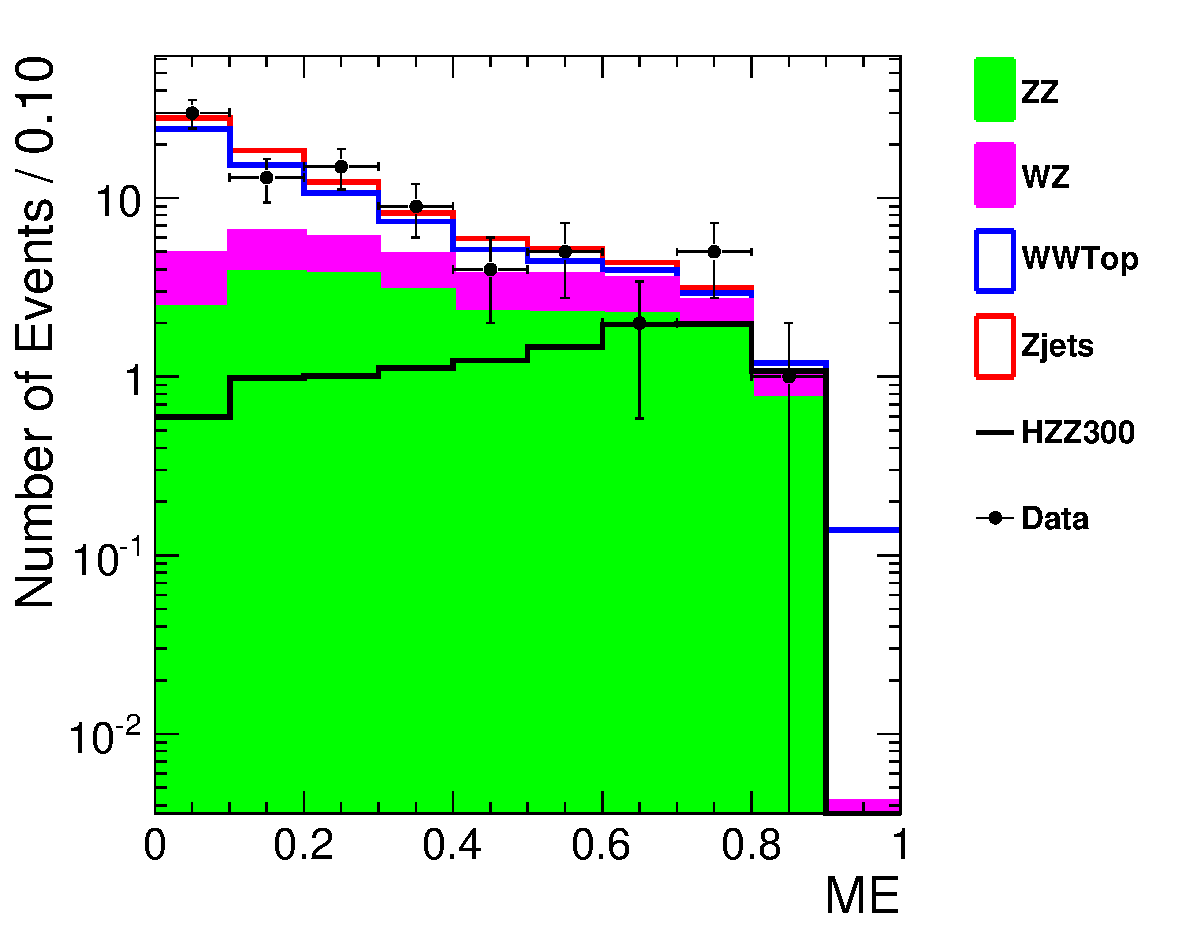
\includegraphics[width=0.4\textwidth,angle=0]{figures/ME_mH300_ee_stack_log.pdf}} 
   \subfigure[]{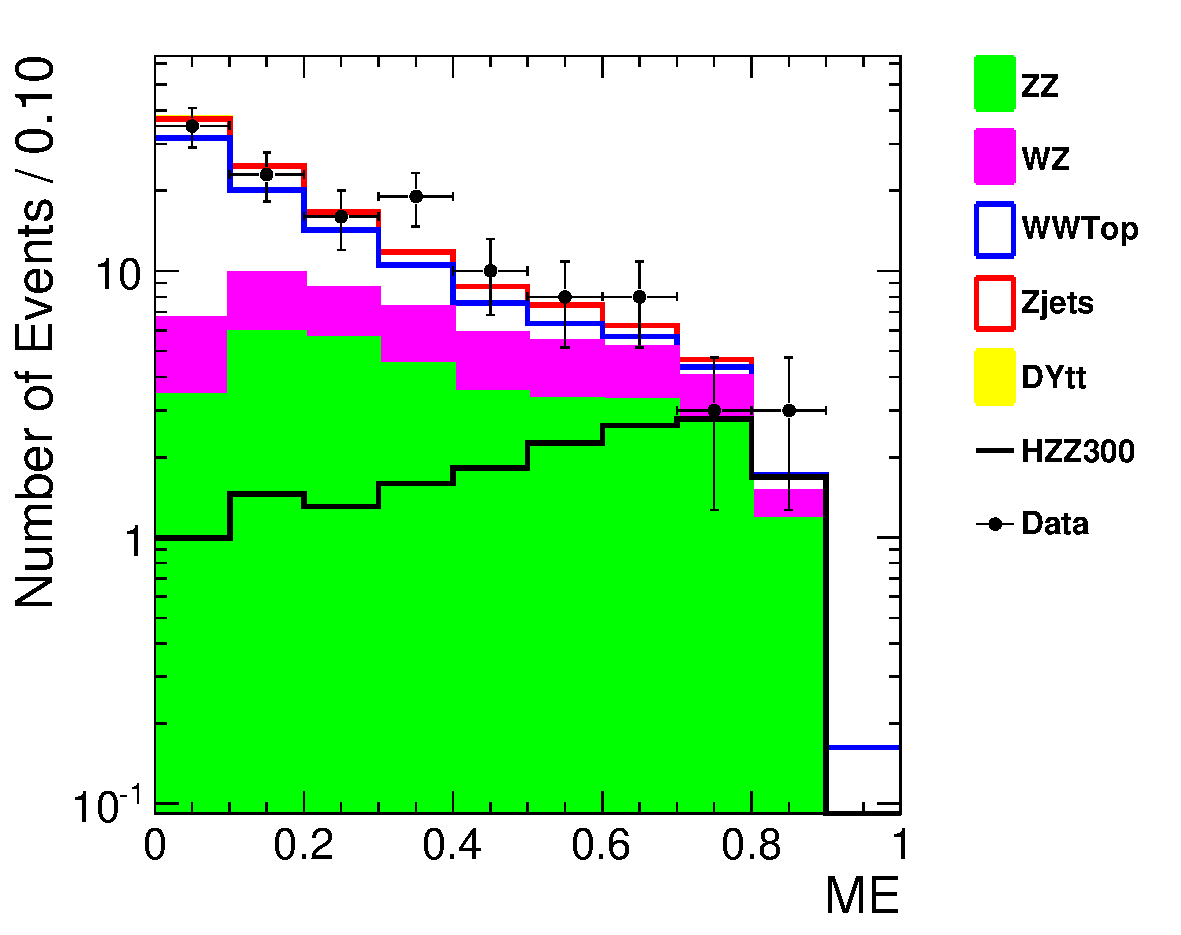
\includegraphics[width=0.4\textwidth,angle=0]{figures/ME_mH300_mm_stack_log.pdf}} \\ 
   \caption{The matrix element output distribution for Higgs signal and background events 
for \mHi=300 $\GeVcc$ in ee (a) and $\mu\mu$ final state (b) after the higgs dependent selections. 
The distributions are normalized to \intlumi with the background scaled by the data-to-mc ratios derived from data.}
   \label{fig:histo_me_300_5fb}
\end{center}
%\end{figure}

%\begin{figure}[!ht]
\begin{center}
   \subfigure[]{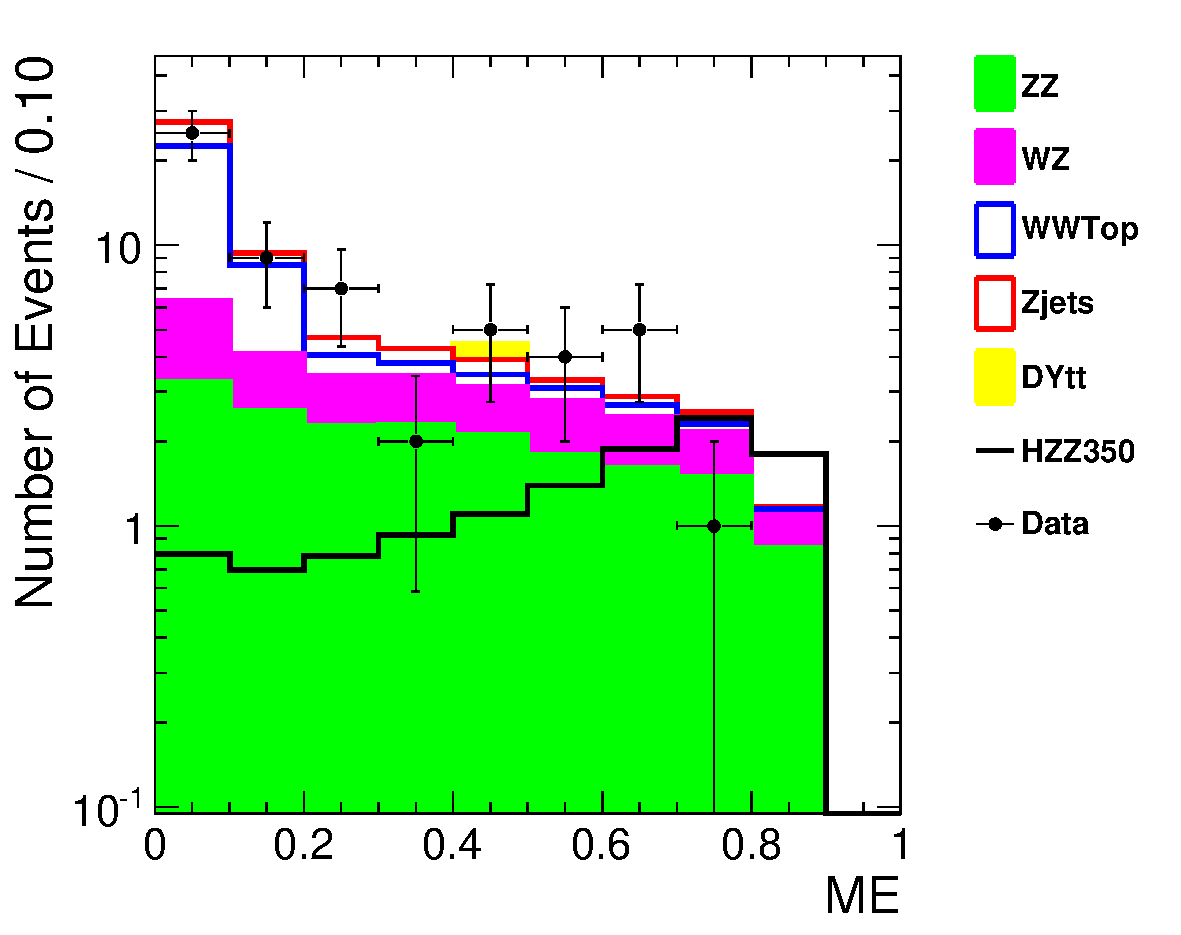
\includegraphics[width=0.4\textwidth,angle=0]{figures/ME_mH350_ee_stack_log.pdf}} 
   \subfigure[]{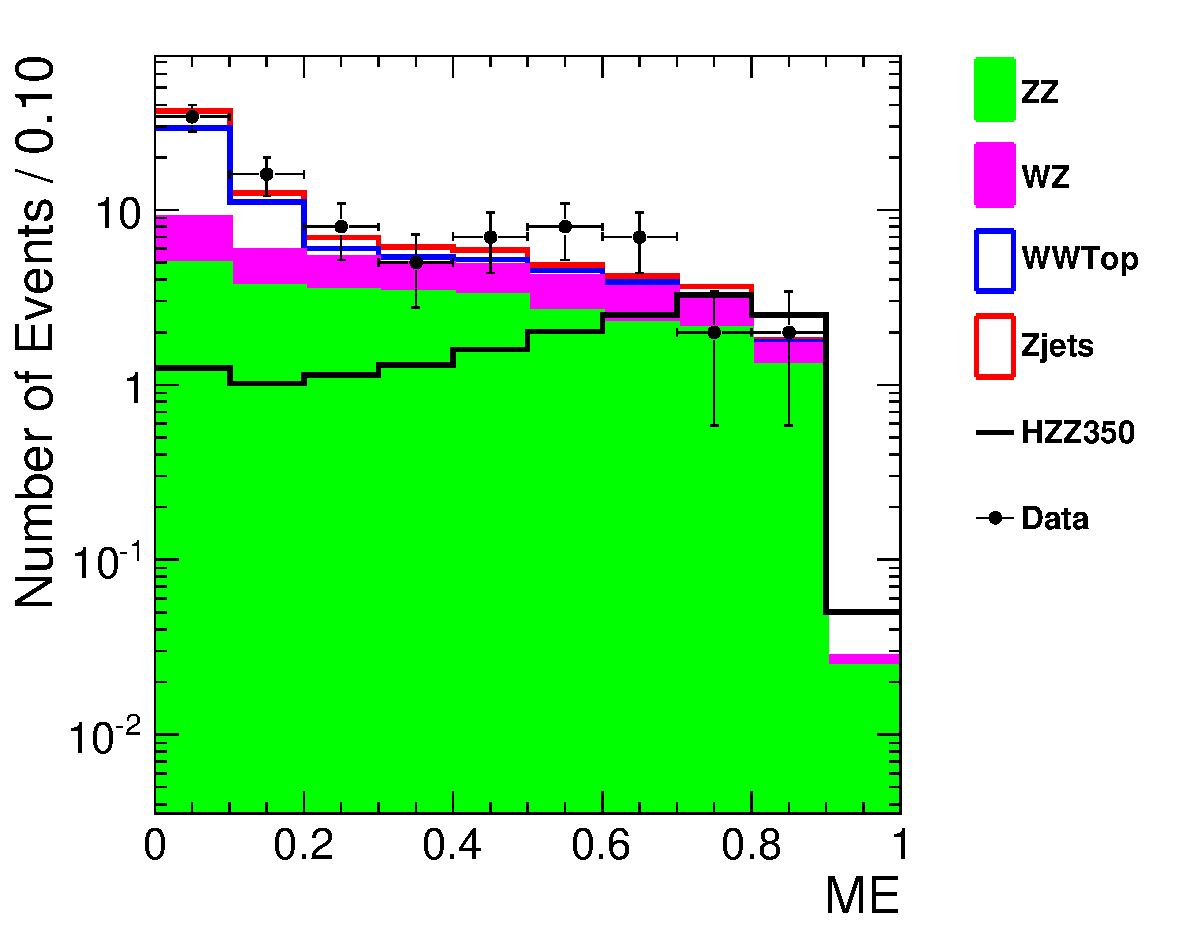
\includegraphics[width=0.4\textwidth,angle=0]{figures/ME_mH350_mm_stack_log.pdf}} \\ 
   \caption{The matrix element output distribution for Higgs signal and background events 
for \mHi=350 $\GeVcc$ in ee (a) and $\mu\mu$ final state (b) after the higgs dependent selections. 
The distributions are normalized to \intlumi with the background scaled by the data-to-mc ratios derived from data.}
   \label{fig:histo_me_350_5fb}
\end{center}
\end{figure}

\begin{figure}[!ht]
\begin{center}
   \subfigure[]{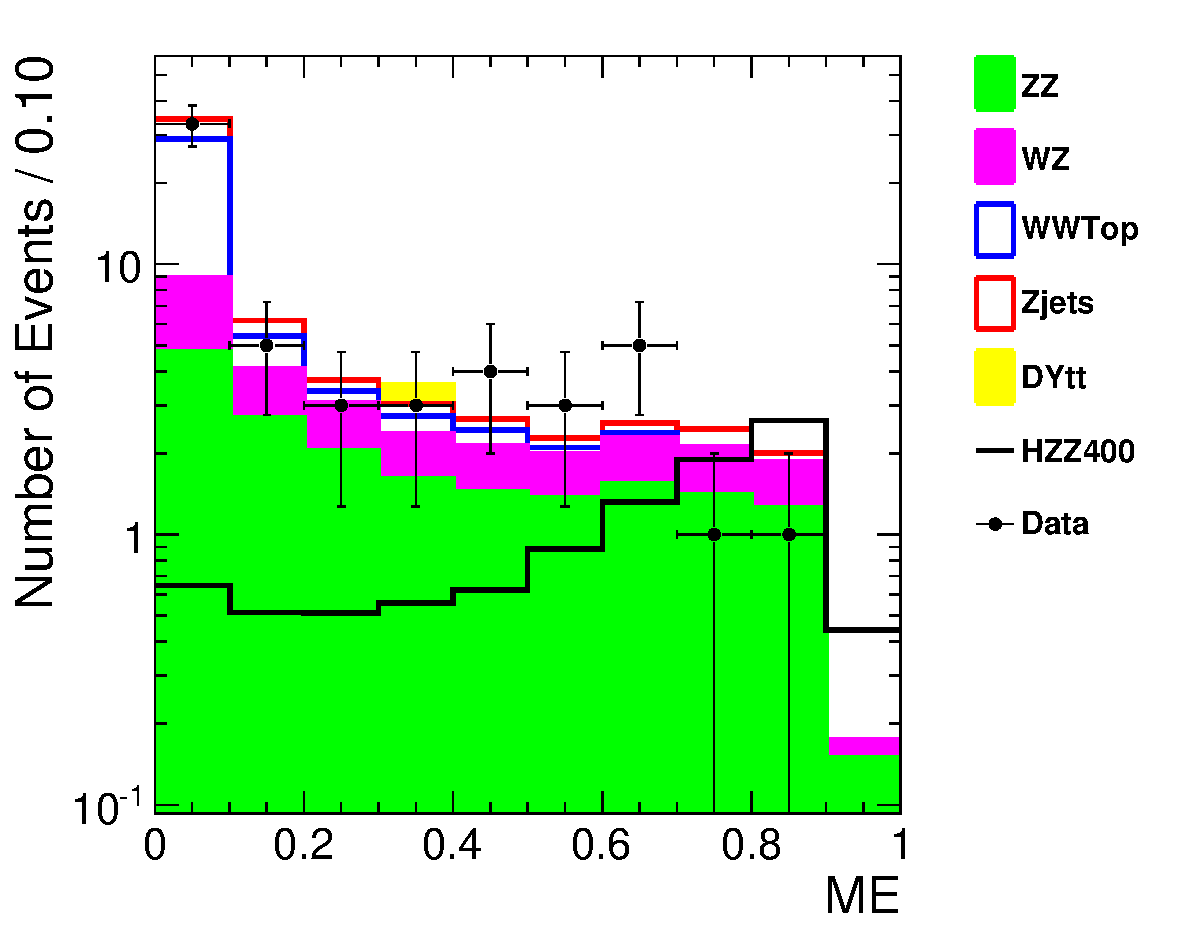
\includegraphics[width=0.4\textwidth,angle=0]{figures/ME_mH400_ee_stack_log.pdf}} 
   \subfigure[]{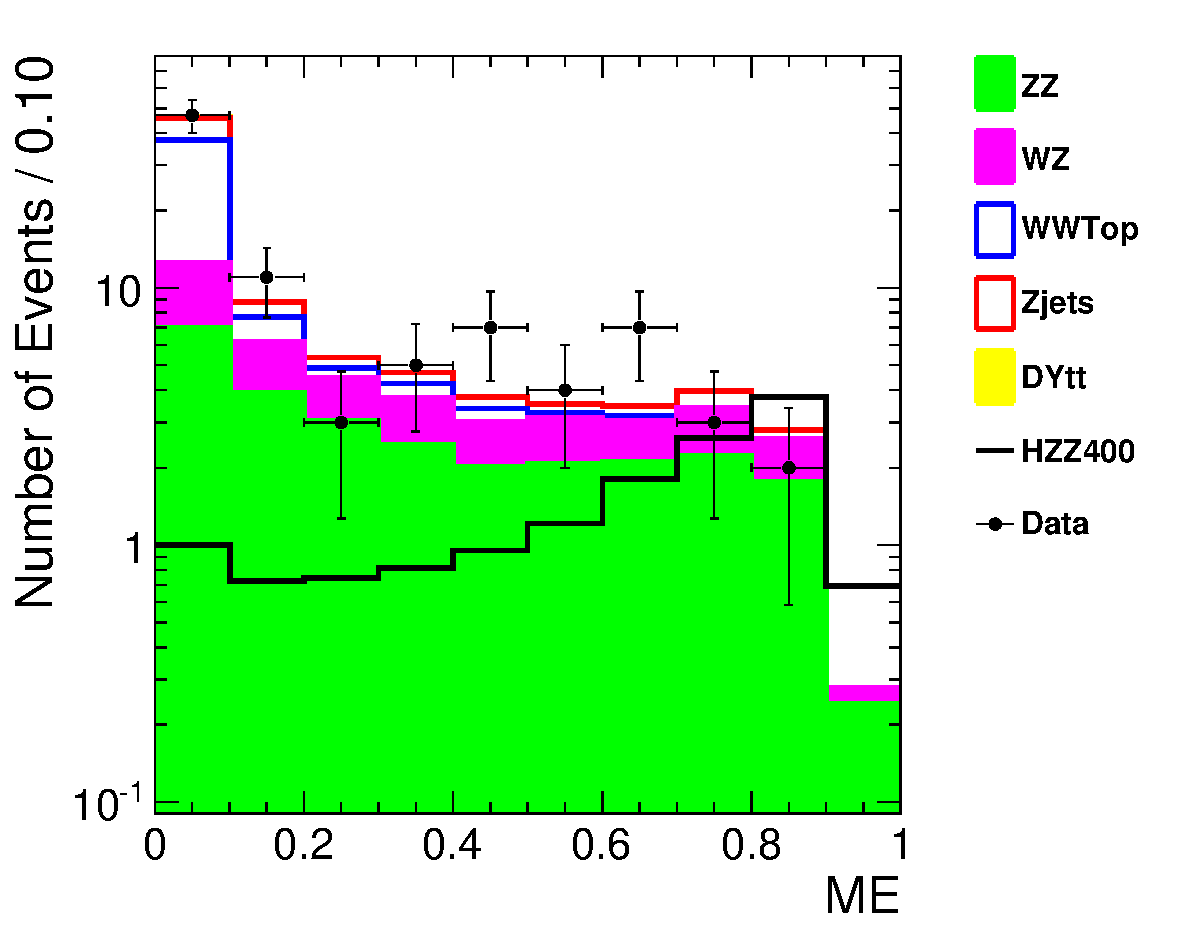
\includegraphics[width=0.4\textwidth,angle=0]{figures/ME_mH400_mm_stack_log.pdf}} \\ 
   \caption{The matrix element output distribution for Higgs signal and background events 
for \mHi=400 $\GeVcc$ in ee (a) and $\mu\mu$ final state (b) after the higgs dependent selections. 
The distributions are normalized to \intlumi with the background scaled by the data-to-mc ratios derived from data.}
   \label{fig:histo_me_400_5fb}
\end{center}
\end{figure}


\begin{figure}[!ht]
\begin{center}
   \subfigure[]{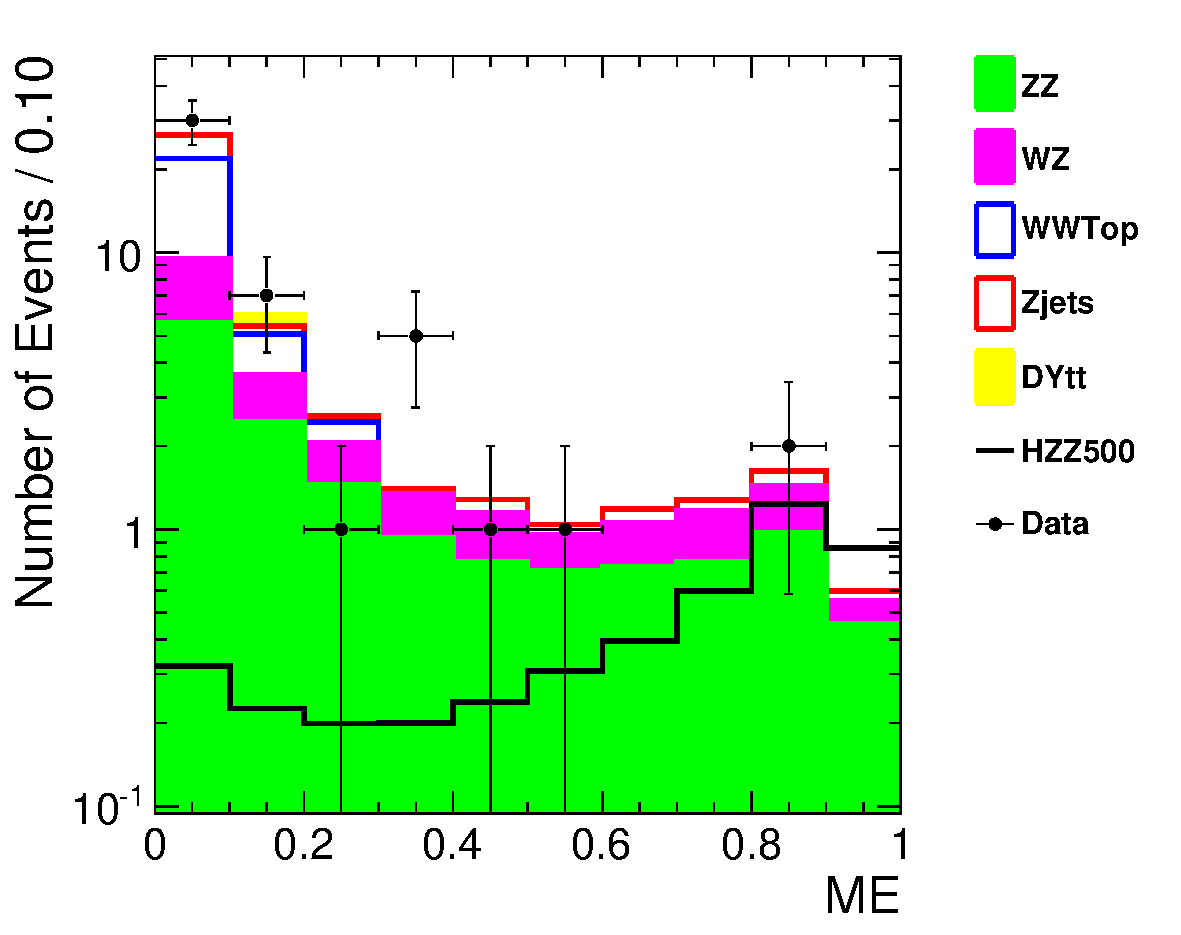
\includegraphics[width=0.4\textwidth,angle=0]{figures/ME_mH500_ee_stack_log.pdf}} 
   \subfigure[]{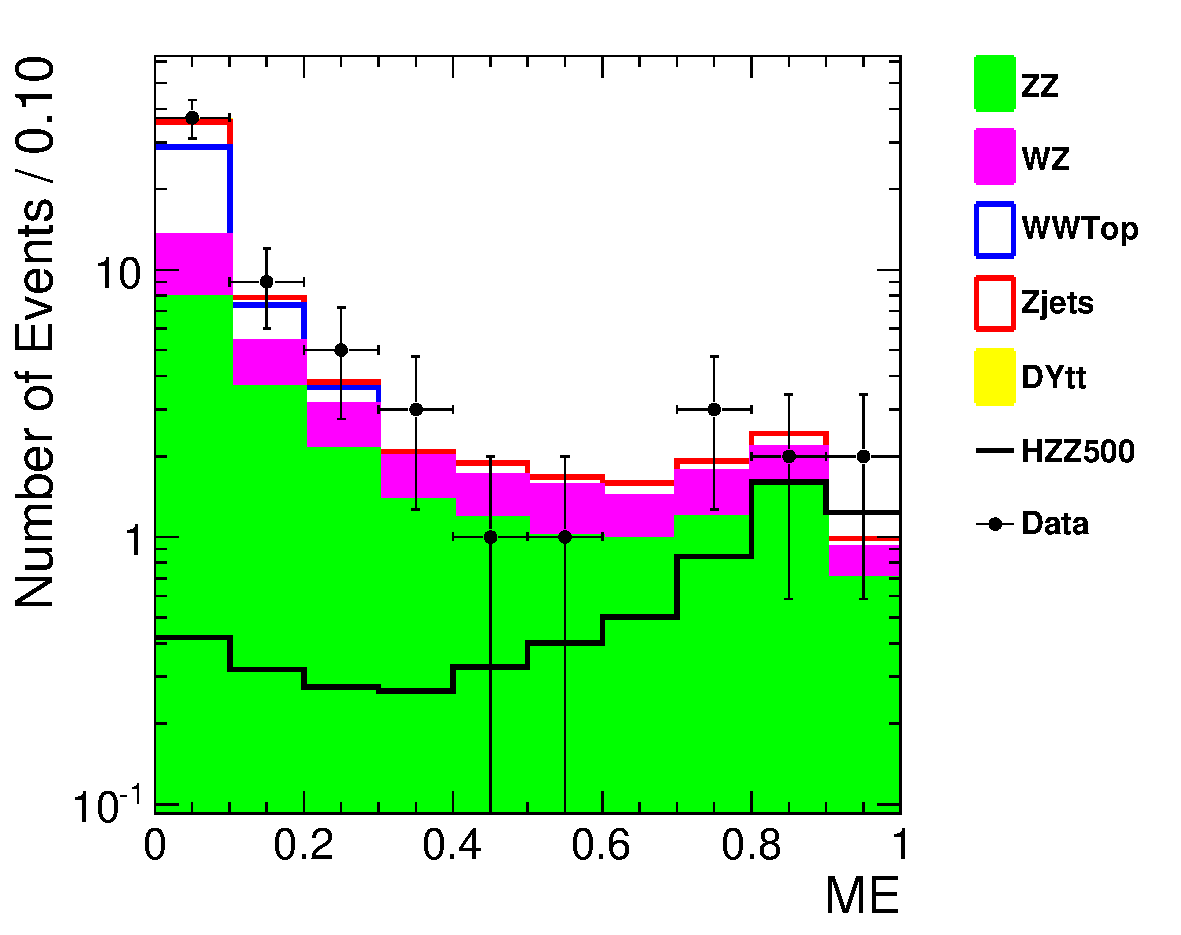
\includegraphics[width=0.4\textwidth,angle=0]{figures/ME_mH500_mm_stack_log.pdf}} \\ 
   \caption{The matrix element output distribution for Higgs signal and background events 
for \mHi=500 $\GeVcc$ in ee (a) and $\mu\mu$ final state (b) after the higgs dependent selections. 
The distributions are normalized to \intlumi with the background scaled by the data-to-mc ratios derived from data.}
   \label{fig:histo_me_500_5fb}
\end{center}
\end{figure}

\begin{figure}[!ht]
\begin{center}
   \subfigure[]{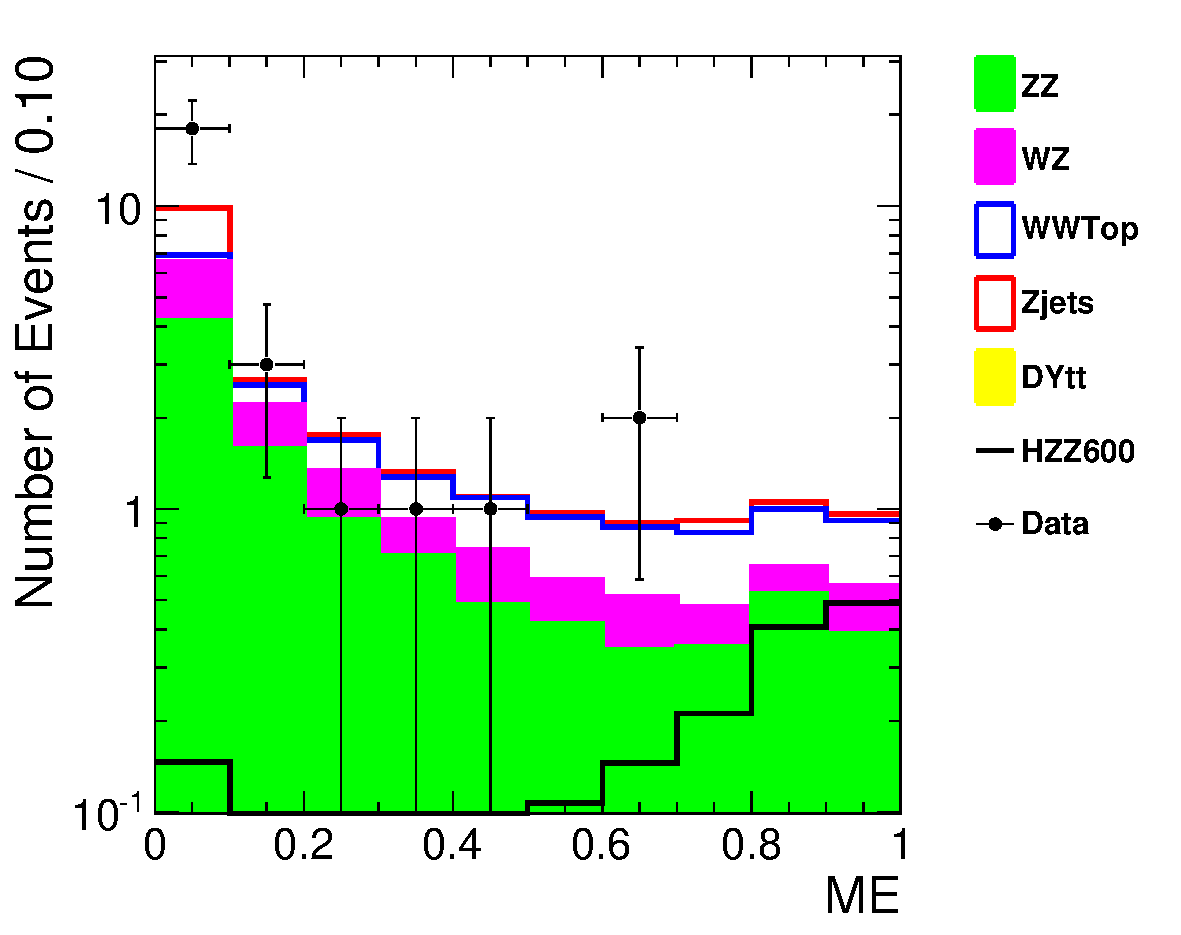
\includegraphics[width=0.4\textwidth,angle=0]{figures/ME_mH600_ee_stack_log.pdf}} 
   \subfigure[]{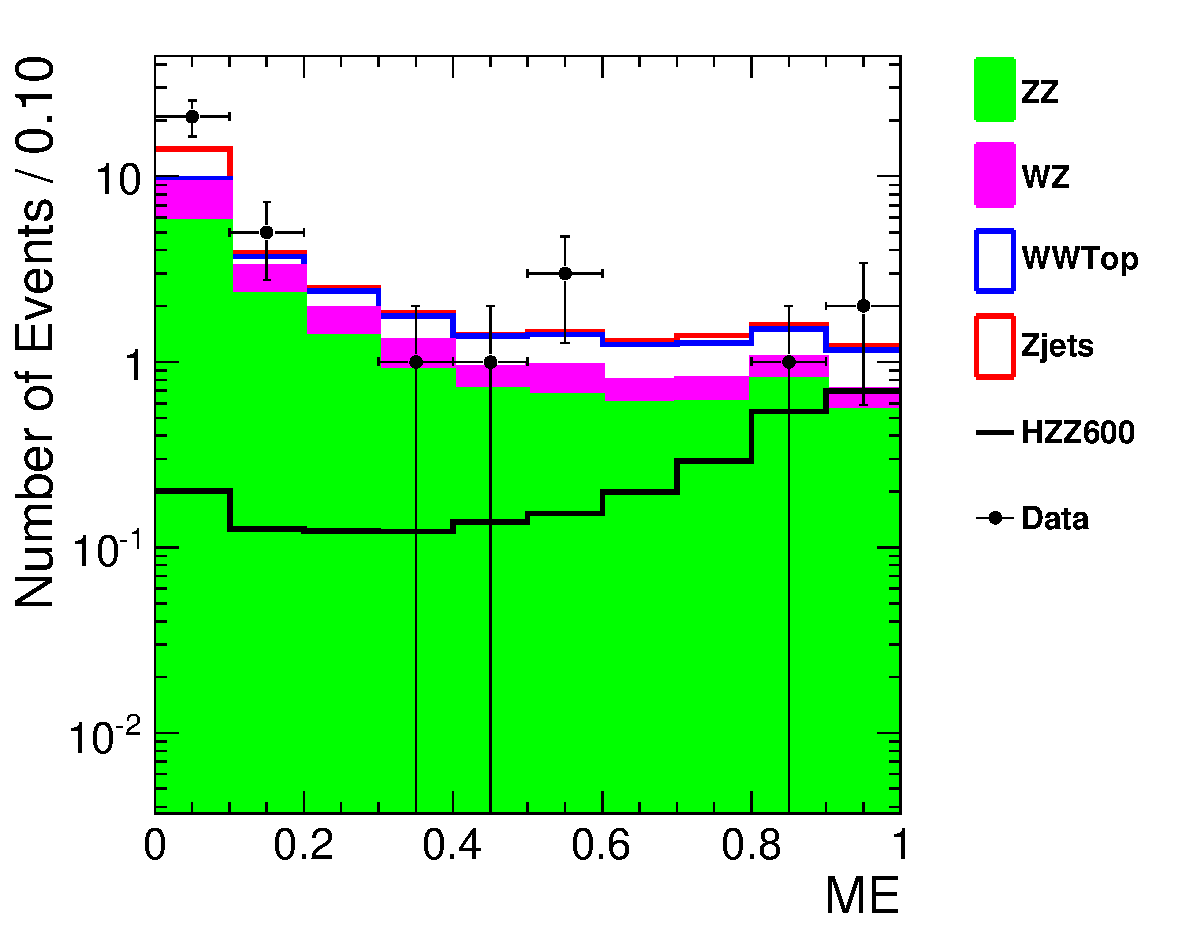
\includegraphics[width=0.4\textwidth,angle=0]{figures/ME_mH600_mm_stack_log.pdf}} \\ 
   \caption{The matrix element output distribution for Higgs signal and background events 
for \mHi=600 $\GeVcc$ in ee (a) and $\mu\mu$ final state (b) after the higgs dependent selections. 
The distributions are normalized to \intlumi with the background scaled by the data-to-mc ratios derived from data.}
   \label{fig:histo_me_600_5fb}
\end{center}
\end{figure}
%%%%%%%%%%%%%%%%%%%%%%



%%%%%%%%%%%%%%%%%%%%%%%%%%%%%
%\begin{table}[!ht]
%\begin{center}
%{\normalsize
%\begin{tabular}{|l|c|cccccc|}
%\hline
%      &  Analysis    & adding          &  adding      &  adding      &  adding      & adding      & adding \\
%mH  &  without     & template        &  $H\to ZZ$   &  Top         &  WW          & WZ          & ZZ \\
%      &  shape syst. & stat. uncert.   &  QCD effect &  shape syst. &  shape syst. & shape syst. & shape syst. \\
%\hline
%250 & 1.62 & 1.71 & 1.69 & 1.70 & 1.73 & 1.72 & 1.71 \\   
%300 & 1.00 & 1.03 & 1.02 & 1.06 & 1.05 & 1.06 & 1.06 \\ 
%350 & 0.70 & 0.71 & 0.71 & 0.72 & 0.72 & 0.72 & 0.72 \\
%400 & 0.70 & 0.70 & 0.70 & 0.70 & 0.70 & 0.71 & 0.71 \\
%500 & 1.26 & 1.28 & 1.28 & 1.28 & 1.29 & 1.29 & 1.30 \\
%600 & 2.79 & 2.88 & 2.84 & 2.84 & 2.86 & 2.88 & 2.87 \\
%\hline
%\end{tabular}
%}
%\caption{Comparison of the median expected cross section ratio limits as a function 
%of the Higgs mass between shape analysis without and with accouting for the 
%shape variation systematics. The results on the various sources are added sequentially 
%to study the impact of each source. Note that the statistical precision on the limits 
%here are around 1\%. }
%\label{tab:mva_meshape_detail}
%\end{center}
%\end{table}
%%%%%%%%%%%%%%%%%%%%%%%%%%%%%


%%%%%%%%%%%%%%%%%%%%%%%%%%%%%
\begin{figure}[!htbp]
\begin{center}
   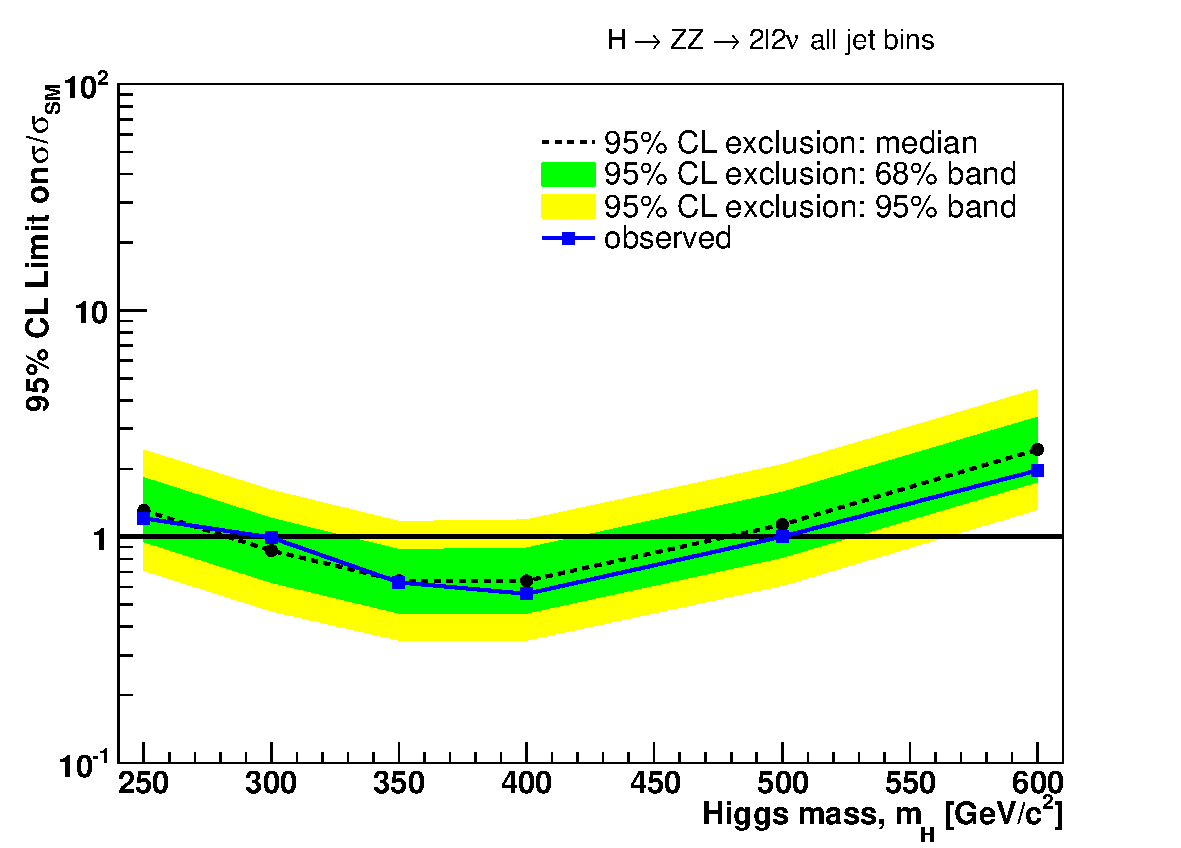
\includegraphics[width=0.8\textwidth]{figures/limits_meshape_5fb.pdf}
   \caption{ The expected upper limits at 95\% C.L. for \intlumi\ of data for the matrix element output shape based (right) analyses. 
	The matrix element output shape analysis includes all the shape systematics. }
   \label{fig:limits_meshape_5fb}
\end{center}
\end{figure}
%%%%%%%%%%%%%%%%%%%%%%%%%%%%%
